\documentclass[10pt,letterpaper]{article}
\usepackage[margin=.75in]{geometry}
\usepackage{amsmath}
\usepackage{amssymb}
\usepackage{fancyhdr}
\usepackage{pgfplots}
\usepackage[shortlabels]{enumitem}
\usepackage{listings}
\usepackage[document]{ragged2e}
\usepackage{setspace}
\graphicspath{ {./} }
\onehalfspacing

\author{Orkun Akyol}
\title{Statistics For Data Science: HW 2}

\pagestyle{fancy}
\renewcommand{\headrulewidth}{0pt}
\renewcommand{\footrulewidth}{0pt}
\lstset{frame=tb,
  aboveskip=3mm,
  belowskip=3mm,
  showstringspaces=false,
  columns=flexible,
  basicstyle={\small\ttfamily},
  numbers=none,
  numberstyle=\tiny\color{gray},
  breaklines=true,
  breakatwhitespace=true,
  tabsize=3
}
\setlength{\headheight}{25pt}
\fancyhf{}
\rhead{
    Rajan Puri | Shameem Ahmed Khan | Orkun Akyol | Gabriel Brown \\
    Statistics | Winter 2024\\
    Homework 2
}
\rfoot{\thepage}

\begin{document}

\paragraph{Q1}
To use the inverse transform sampling, first we need to calculate the cumulative distribution function of \( X \). 
\[
F(x) = \int_{0}^{x} \frac{4te^{-t^2}}{(e^{-t^2}+1)^2} \,dt
\]    
To calculate the integral, let us make the substitution \( u = e^{-t^2}+1 \). Then,
\[
du = -2te^{-t^2} \,dt \Rightarrow dt = \frac{du}{-2te^{-t^2}}
\]
Rearranging gives:
\[
F(x) = -2 \int_{0}^{x} \frac{1}{u^2} \, du = 2\left[-\frac{1}{u}\right]_{0}^{x} = 2\left(\frac{1}{e^{-x^2}+1} - \frac{1}{1}\right) 
\]
Thus, we have:
\[
F(x) = \begin{cases}
0 & \text{if } x < 0\\
\frac{2}{e^{-x^2}+1}-1 & \text{if } x \ge 0
\end{cases}
\]

Now, let us calculate the inverse of the CDF:
\[
y = \frac{e^{t^2}-1}{e^{t^2}+1}
\]
This leads to:
\[
e^{t^2}(y + 1) = 1 + y
\]
\[
e^{t^2} = \frac{1 + y}{y + 1}
\]
Taking the natural log:
\[
t^2 = \ln\left(\frac{1+y}{y-1}\right)
\]
\[
t = \sqrt{\ln\left(\frac{1+y}{y-1}\right)}
\]
Since the PDF is \( 0 \) for \( x<0 \), we are interested in the positive root. For sampling from the CDF, the outputs and plots are provided in HW2Q1.ipynb.

\paragraph{Q2}
Let \( X \sim N(0, 1) \) and define \( Y = g(X) \), where \( g(x) = \tan^{-1}(x) \) for \( x \in \mathbb{R} \).
\begin{itemize}
    \item Draw a sample \( X \sim N(0, 1) \) of size \( n = 10^5 \) and plot \( g(X) \) as a histogram.
    \item Derive the probability density function of random variable \( Y \). Plot this alongside the (appropriately normalized) histogram obtained in part (a).
\end{itemize}
Hint: In Python, you can use \texttt{numpy.random.normal(m,sigma,size=n)} to draw a sample containing \( n \) entries from the Gaussian distribution \( N(m, \sigma^2) \).

\lstset{language=Python}
\begin{lstlisting}
#Here is the code for your reference, you can check the graphs in HW2Q2.ipynb

#first part of the question 
import numpy as np
import matplotlib.pyplot as plt

np.random.seed(0)

# Sample size which was mentioned
n = 10**5
X = np.random.normal(0, 1, n)
Y = np.arctan(X)

# Plot the histogram of Y
plt.figure(figsize=(10, 6))
plt.hist(Y, bins=100, density=True, alpha=0.7, color='blue', edgecolor='black')
plt.title('Histogram of Y = arctan(X) where X ~ N(0, 1)')
plt.xlabel('Y')
plt.ylabel('Density')
plt.grid()
plt.show()




#second part of question
def fun(y):
    return (1 / np.sqrt(2 * np.pi)) * np.exp(-np.tan(y)**2 / 2) * (1 / np.cos(y)**2)

y_values = np.linspace(-np.pi/2 + 0.01, np.pi/2 - 0.01, 1000)
pdf_values = fun(y_values)

# Plotting
plt.figure(figsize=(10, 6))
plt.hist(Y, bins=100, density=True, alpha=0.5, color='blue', edgecolor='black', label='Histogram of Y')
plt.plot(y_values, pdf_values, color='red', label='PDF of Y', linewidth=2)
plt.title('Histogram and PDF of Y = arctan(X) where X ~ N(0, 1)')
plt.xlabel('Y')
plt.ylabel('Density')
plt.legend()
plt.grid()
plt.show()
\end{lstlisting}

\paragraph{Q3}
\textbf{Let $X, Y \sim U(0,1)$ be independent random variables and define $Z = max(X, Y^2)$}
\begin{enumerate}[(a)]
    \item \textbf{derive the probability density function of Z.}\\
    $F_Z(z) = P(Z\leq z) = P(max(X, Y^2) \leq z) = P(X \leq z \text{ and } Y^2 \leq z)$\\
    X and Y are independent $\implies F_Z(z) = P(X\leq z) \dot P(Y^2\leq z) = P(X\leq z) \dot P(Y\leq \sqrt{z}) = z\sqrt{z}$ for $0\leq z \leq 1$\\
    $f_Z(z) = \frac{d}{dz} F_Z(z) = \frac{3\sqrt{z}}{2}$\\
    therefore, the PDF of Z is 
    $$f_Z(z) = \begin{cases}
    0 & \text{ if } x < 0\\
    \frac{3\sqrt{z}}{2} & \text{ if } 0 \leq x \leq 1\\
    0 & \text{ if } x > 1
\end{cases}$$
    \item \textbf{Draw a sample of size $n = 10^5$ from the probability distribution of Z and visualize the sample as a histogram. Plot the probability density you obtained in part (a) alongside the (appropriately normalized) histogram.}
    See HW3Q3.ipynb to run code\\
    \begin{lstlisting}[language=Python]
import numpy as np
import matplotlib.pyplot as plt
import seaborn as sns

X = np.random.uniform(0, 1, 10**5)
Y = np.random.uniform(0, 1, 10**5)
Z = np.maximum(X, Y**2)

sns.histplot(Z, bins=50, kde=False, stat='density', color='blue', label="Sampled Z")
z_values = np.linspace(0, 1, 1000)
pdf_values = (3 / 2) * np.sqrt(z_values)

plt.plot(z_values, pdf_values, 'r-', label="pdf of Z", linewidth=2)

plt.title("Histogram of 10^5 samples of Z and PDF")
plt.xlabel("Z")
plt.ylabel("Density")
plt.legend()

plt.show()
\end{lstlisting}
output:
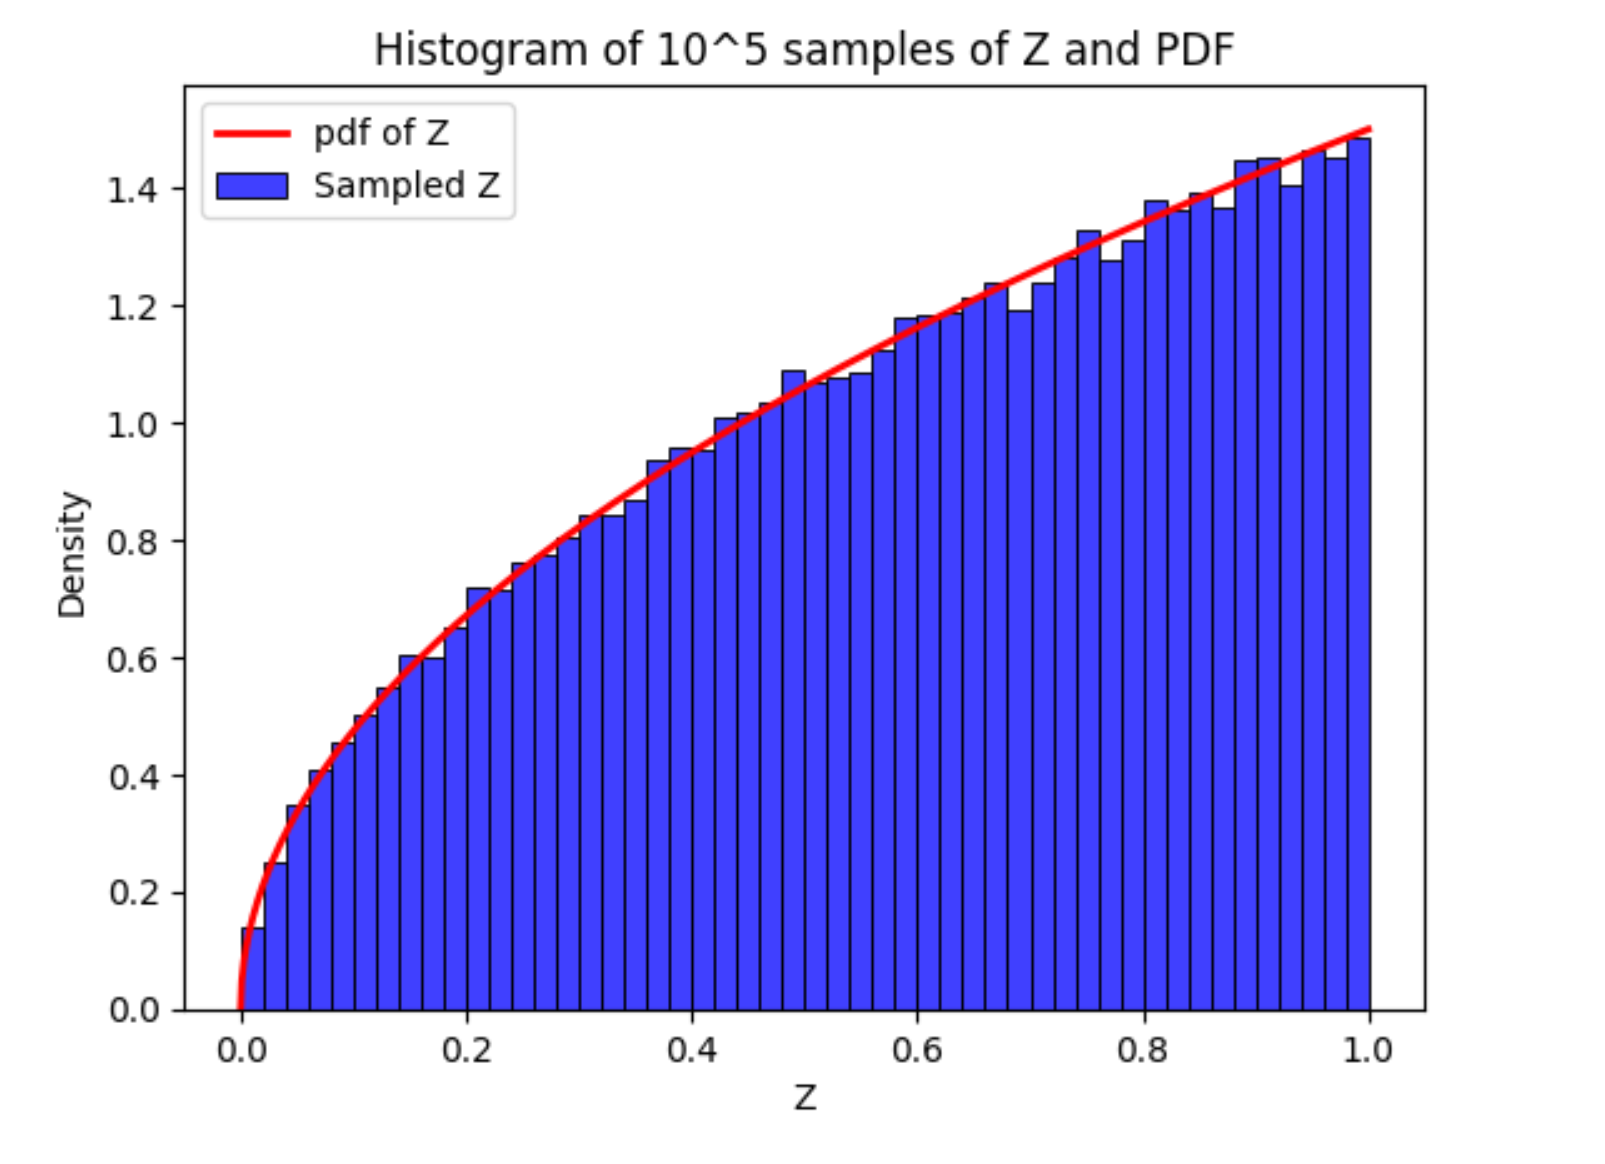
\includegraphics[scale=.7]{q3graph.png}\\
\end{enumerate}

\paragraph{Q4}
Let \((X_1, X_2)\) be a joint random variable, and assume that 
\[
(\log X_1, \log X_2) \sim N\left(\begin{pmatrix} 1 \\ 1 \end{pmatrix}, \begin{pmatrix} 2 & -1 \\ -1 & 2 \end{pmatrix}\right).
\]

We aim to derive the joint probability density function (PDF) of \((X_1, X_2)\).

Recall that the bivariate Gaussian distribution \(Y \sim N(\mu, C)\) for vector \(\mu \in \mathbb{R}^2\) and a symmetric, positive definite matrix \(C \in \mathbb{R}^{2 \times 2}\) has the probability density function given by:
\[
f_Y(y) = \frac{1}{2\pi \sqrt{\det C}} \exp\left(-\frac{1}{2} (y - \mu)^T C^{-1} (y - \mu)\right), \quad y \in \mathbb{R}^2.
\]



\section*{Step 1: Analysis of Provided Information}
1. We are given that \((X_1, X_2)\) is a joint random variable, where:
   \begin{itemize}
       \item Mean vector: \(\mu = \begin{pmatrix} 1 \\ 1 \end{pmatrix}\).
       \item Covariance matrix: \(C = \begin{pmatrix} 2 & -1 \\ -1 & 2 \end{pmatrix}\).
   \end{itemize}
   Let \((Y_1, Y_2) = (\log X_1, \log X_2)\), which follows a bivariate normal distribution:

   In other words, \((Y_1, Y_2)\) has a joint Gaussian distribution where each variable has a mean of 1, and the covariance matrix \(C\) defines how the two variables vary and correlate.

\section*{Step 2: Density Function for \(Y\)}
2. The formula for the bivariate density function is given by:
   \[
   f_Y(y) = \frac{1}{2\pi \sqrt{\det C}} \exp\left(-\frac{1}{2} (y - \mu)^T C^{-1} (y - \mu)\right),
   \]
   where \(\mu\) is the mean vector, and \(C\) is the covariance matrix. This formula has several components:
   \begin{itemize}
       \item \(\frac{1}{2\pi \sqrt{\det C}}\): A normalization constant that ensures the density integrates to 1 over the entire space.
       \item \(\exp\left(-\frac{1}{2} (y - \mu)^T C^{-1} (y - \mu)\right)\): An exponential that represents the Gaussian “shape” based on the distance between \(y\) and the mean, weighted by the inverse of the covariance matrix \(C\).
   \end{itemize}
   Here, \(y\) represents a particular realization of the random variables.

3. To find the value of \(\det C\), we calculate the determinant of the covariance matrix:
   \[
   \det C = 2 \cdot 2 - (-1)(-1) = 4 - 1 = 3.
   \]

4. To compute the Gaussian formula, we need the inverse of the covariance matrix \(C^{-1}\). The inverse is calculated as:
   \[
   C^{-1} = \frac{1}{\det C} \begin{pmatrix} 2 & 1 \\ 1 & 2 \end{pmatrix} = \frac{1}{3} \begin{pmatrix} 2 & 1 \\ 1 & 2 \end{pmatrix}.
   \]

\section*{Step 3: Substitute the Values into the Density Function}
5. Now that we have \(\det C\) and \(C^{-1}\), we can plug these into the density function:
   \[
   f_Y(y) = \frac{1}{2\pi \sqrt{3}} \exp\left(-\frac{1}{2} (y - \begin{pmatrix} 1 \\ 1 \end{pmatrix})^T \frac{1}{3} \begin{pmatrix} 2 & 1 \\ 1 & 2 \end{pmatrix} (y - \begin{pmatrix} 1 \\ 1 \end{pmatrix})\right).
   \]

6. To simplify the exponent, we expand the expression inside the exponent. The quadratic form in the exponent simplifies to:
   \[
   (y - \begin{pmatrix} 1 \\ 1 \end{pmatrix})^T \frac{1}{3} \begin{pmatrix} 2 & 1 \\ 1 & 2 \end{pmatrix} (y - \begin{pmatrix} 1 \\ 1 \end{pmatrix}).
   \]
   This term measures the “distance” from \(y\) to the mean \(\mu\), adjusted by the covariance structure.

\section*{Step 4: Transform the Density of \(X\)}
7. Change of Variables: We know that \(Y_1 = \log X_1\) and \(Y_2 = \log X_2\), so \(Y\) can be thought of as a transformed version of \(X\). The relationship between the densities \(f_X\) and \(f_Y\) is given by:
   \[
   f_X(x_1, x_2) = f_Y(y_1, y_2) \cdot \left| \det(J) \right|,
   \]
   where \(J\) is the Jacobian determinant that accounts for the change in “volume” when transforming from \(Y\) to \(X\).

8. Compute the Jacobian Determinant: The Jacobian matrix of the transformation where \(X_1 = e^{Y_1}\) and \(X_2 = e^{Y_2}\) is:
   \[
   J = \begin{pmatrix}
   \frac{\partial X_1}{\partial Y_1} & \frac{\partial X_1}{\partial Y_2} \\
   \frac{\partial X_2}{\partial Y_1} & \frac{\partial X_2}{\partial Y_2}
   \end{pmatrix} = \begin{pmatrix}
   e^{Y_1} & 0 \\
   0 & e^{Y_2}
   \end{pmatrix}.
   \]
   The determinant is:
   \[
   \det(J) = e^{Y_1} e^{Y_2} = X_1 X_2.
   \]

9. Substitute Everything into \(f_X\): Now, we substitute \(f_Y\) and the Jacobian determinant into the density function for \(X\):
   \[
   f_X(x_1, x_2) = f_Y(\log x_1, \log x_2) \cdot (x_1 x_2).
   \]


\end{document}

